\chapter{时间网与实际制造系统结合}

\section{变迁和库所上均有时延的时间Petri网}
假设存在一个场景,机械臂需要从加工腔中取走一个工件放入另一个加工腔,
工件在加工腔中加工需要时间,机械臂移动也需要时间。
如果将加工腔看作库所,工件看作托肯,机械臂的动作看作变迁,
则意味着托肯进入某库所后等待一段时间,
之后变迁开始计时一段时间后发射,
将此托肯移入另一个库所中。

因此需要一种新的时间Petri网模型,将TTPN和TPPN结合起来,本文提出了一种新的时间Petri网子类,时间变迁库所网(Time Transition Place Petri Net,TTPPN),
解决了这种场景下的建模问题。

TTPPN需要在变迁和库所上都添加时间区间。库所上的时间区间表示进入此库所的托肯,至少需要等待一段时间才能被取走,但不能驻留过长的时间。
普通Petri网的使能逻辑中某个库所是否使能只需要判断此库所中的托肯数是否大于其尝试发射后置变迁输入弧上的权值就行了,
也就是要保证库所中有足够的托肯能被取走。
但TTPPN库所的使能还需要看托肯上的时钟,
因为在TPPN中,托肯能否被取走,还需要判断托肯的停留时间是否满足了库所上的时间限制。
因此TTPPN库所能否使能,需要看此库所中满足此库所时间限制的托肯的个数是否不低于其尝试发射后置变迁输入弧上的权值。

\textbf{定义3.1}\textbf{:}
一个TTPPN是一个七元组$Z=(P,T,F,W,M_{0},I_{p},I_{t})$,其中:

1. 五元组$(P,T,F,W,M_{0})$是一个基本Petri网;

2. $I_{p}:P \rightarrow (\mathbb{Q}_{0}^{+} \cup 0) \times (\mathbb{Q}_{0}^{+} \cup {\infty})$,$p_{i} \rightarrow I(p_{i})=[a_{i},b_{i}], 0 \leq a_{i} \leq b_{i} $;

3. $I_{t}:P \rightarrow (\mathbb{Q}_{0}^{+} \cup 0) \times (\mathbb{Q}_{0}^{+} \cup {\infty})$,$t_{i} \rightarrow I(t_{i})=[a_{i},b_{i}], 0 \leq a_{i} \leq b_{i} $。

在TTPN中,变迁一旦使能,其上的时钟便会开始计时。在TTPPN中也是如此。
当此变迁的所有前置库所都使能的那一瞬间,此变迁的时钟开始计时。

在实际的制造系统中,完成工序的耗时是一个衡量控制策略的重要指标。
Petri网的变迁表示的是此系统能执行的动作。
为了让系统完成任务所执行的一系列的动作的耗时尽可能短,则要避免不必要的时间开销。
这意味着,变迁的发射应该尽可能早,变迁上的时钟不允许有无意义的计时。

为了实现这个需求,发射逻辑应该分为3部分:变迁发射前的逻辑、变迁发射的逻辑、变迁发射后的逻辑。
某变迁如果满足库所使能,并且需要被发射,须要按顺序执行完这3个逻辑。

\begin{algorithm}[H]
    \caption{变迁发射逻辑}
    \hspace*{0.02in} {\bf 输入:} 
    变迁库所时间网$TTPPN$,变迁库所时间网的标识$Marking$,准备发射的变迁$t$\\
    \hspace*{0.02in} {\bf 输出:}
	变迁$t$发射后到达的新标识$next$
    \begin{algorithmic}[1]
		\State $next \leftarrow $将$Marking$克隆一份
		\State $beforeTlanuch(TTPPN,next,t)$ //变迁发射前的逻辑
		\State $tlanuch(TTPPN,next,t)$ //变迁发射的逻辑
		\State $afterTlanuch(TTPPN,next,t)$ //变迁发射后的逻辑
		\State 返回$next$
    \end{algorithmic}
\end{algorithm}

变迁发射前的逻辑要实现两个目标:1、计算出使此变迁使能的最短时间。2、从对应库所中删除被此变迁取走的托肯。
变迁如果要使能,则其前置库所中需要有足够多完成计时的托肯。
因此变迁使能的最短时间为此变迁所有前置库所中,所有被取走托肯中计时离时间限制最长的那段时间。
如果将时钟改为倒计时,此时间应该为被取走的托肯中倒计时最长的那个时间。
为了避免消耗不必要的时间,对于特定库所,取走的托肯应该是最先完成倒计时的那一批。


\begin{algorithm}[H]
	\caption{变迁发射前的逻辑}
	\label{alg3-2}
	\begin{algorithmic}
		\Procedure{beforeTlanuch}{$TTPPN$,$next$,$t$}
		\ForAll{$p \in {\bullet}t$}
		\State $needGetCount \leftarrow Pre(p,t)$
		\State $minTime \leftarrow$ 标识$next$库所$p$中第$needGetCount$的时钟计时 
		\State $time \leftarrow max(time,minTime) $// $time$为使变迁$t$使能的最短时间
		\ForAll{$token \in TOKEN(p)$} //$TOKEN(p)$ 为库所$p$中的托肯的集合
		\If{$TIME(token) \le minTime$} //$TIME(token)$ 为此token上时钟的计时
		\State 从$TOKEN(p)$中删除$token$
		\EndIf
		\EndFor
		\EndFor
		\EndProcedure
	\end{algorithmic}
\end{algorithm}

按上述流程变迁$t$取托肯时总是从托肯序列的头部取,之后的流程会在托肯序列的尾部放入托肯。
而托肯在库所中停留会导致托肯时钟倒计时。
因此托肯序列必然是升序的。

此处托肯序列选取何种数据结构实现会影响到算法效率。
基于上述分析对托肯序列会有两种操作:
从序列头部删除托肯、从序列尾部添加托肯。
上述需求有两种实现方式:
链表、循环数组。

如果使用链表,即需要定义节点结构。
节点由两部分组成:托肯倒计时时钟、下一个节点的地址。
这将带来以下两个缺陷。

\begin{figure}[H]
	\centering
	% Requires \usepackage{graphicx}
	\includegraphics[scale=1.00,angle=0]{figures/托肯序列_链表.pdf}\\
	\caption{托肯序列的链表实现}
\end{figure}

为了将托肯连接成串,额外存储了大量地址信息。
如果地址和托肯时钟选取相同的数据类型,那么整个数据结构只有一半的有效信息。

当托肯被移除后,此节点便失去引用成为内存垃圾。
清理内存垃圾会带来时间开销。
添加新的托肯需申请新的托肯节点,申请内存亦会带来时间开销。
因此从时间和空间来看,链表这种数据结构实现托肯序列的功能并不高效。

本算法使用循环数组来实现此功能。
预先申请固定长度的数组,并保存头尾两个指针。
当删除托肯时头指针向前移动,如果已经移动到数组尾部,则从头开始。
当添加托肯时,尾指针向前移动,如果已经移动到数组尾部,则从头开始。
当尾指针追上头指针时,意味着数组已满。
需重新申请更大的数组,并将数据移入完成扩容。

\begin{figure}[H]
	\centering
	% Requires \usepackage{graphicx}
	\includegraphics[scale=1.00,angle=0]{figures/托肯序列_循环数组.pdf}\\
	\caption{托肯序列的循环数组实现}
\end{figure}

循环数组中保留的信息只有托肯时钟,并且添加、删除托肯时如不发生扩容,均不会申请新内存。
如果发生扩容,也是一次申请连续内存,效率高于链表的每次申请单个节点。

变迁发射的逻辑要实现两个目标:1、计算出此变迁发射的总耗时。2、更新其他使能变迁的时钟。
变迁发射的总耗时即为之前求出的变迁使能的最短时间加上此变迁上的时钟。
但是其他变迁有可能在此变迁发射的整个过程中(包过为了让此变迁使能,之前托肯的倒计时过程)使能计时了,
因此需要在此环节一并更新他们的时钟。
这意味着需要对此时库所使能的变迁计算其使能的最短时间,其计算逻辑与变迁发射前的逻辑中的类似。

变迁发射的逻辑是三段逻辑中最为繁琐的,库所时间网和变迁时间网的特点都会在这段逻辑上体现出来。
在变迁时间网中,变迁发射后所有使能变迁是同步开始继续计时的,但结合上库所时间网变迁计时存在先后差异。
因此需要计算出其他变迁提前计时的情况,并更新变迁上时钟。

\begin{algorithm}[H]
	\caption{变迁发射时的逻辑}
	\label{alg3-3}
	\begin{algorithmic}
		\Procedure{tlanuch}{$TTPPN$,$next$,$t$}
		\State $timer \leftarrow TIME(t)$ //$TIME(t)$ 为标识$next$变迁$t$上时钟的倒计时的时间数值
		\State $time=time+timer$
		\ForAll{$t_{other} \in T$}
		\If{$t_{other}^{-} \le m$}
		\State $needGetCount \leftarrow Pre(p,t)$
		\State $minTime \leftarrow 库所p中第needGetCount大的时钟计时 $
		\If{$minTime \le time$}
		\State $TIME(t_{other})=TIME(t_{other})-time+minTime$
		\If{$TIME(t_{other}) \le 0$}
		$TIME(t_{other}) = 0$
		\EndIf
		\EndIf
		\EndIf
		\EndFor
		\EndProcedure
	\end{algorithmic}
\end{algorithm}

变迁发射后的逻辑要实现三个目标:1、对此Petri网所有托肯进行计时.2、对需要重置时钟的变迁,重置其时钟。3、对此变迁的后置库所放入托肯。
TTPPN托肯上的时钟是始终在计时的,因此需要对目前Petri网中的托肯上的倒计时时钟减去变迁发射的总耗时。
当某变迁的前置库所被别的变迁取走过托肯,此变迁上的时钟需要被重置。
当前发射的变迁上的时钟也需要被重置。
变迁发射后,其后置库所会被放入托肯,这些新放入的托肯上的倒计时时钟为库所时延。

在实际的制造系统中,并非所有库所上都有时间约束,因此并不需要对Petri网中的所有托肯重新计算时钟。
当某库所上没有时间约束时,应该跳过计时逻辑。
这段优化在实际情况下有显著效果,因为在建模时会加入额外的控制库所,这类库所中的托肯数往往会远高于其他库所,如果不跳过这些托肯的时钟计算,会浪费大量算力。
\begin{algorithm}[H]
	\caption{变迁发射后的逻辑}
	\label{alg3-4}
	\begin{algorithmic}
		\Procedure{afterTlanuch}{$TTPPN$,$next$,$t$}
		\ForAll{$p \in P$}
		\If{标识$next$库所$p$上没有时间约束}
		\State 跳过计时
		\EndIf
		\ForAll{$token \in TOKEN(p)$}
		\State $TIME(token)=TIME(token)-time$
		\If{$TIME(token)<0$}
		\State $TIME(token)=0$
		\EndIf
		\EndFor
		\EndFor
		\ForAll{$p \in$ $^{\bullet}t$}
		\ForAll{$t_{other} \in p^{\bullet}$}
		\State $TIME(t_{other})=0$
		\EndFor
		\EndFor
		\ForAll{$p \in t^{\bullet}$}
		\State $needPutCount \leftarrow Post(p,t)$
		\For{$i \leftarrow 1, needPutCount$}
		\State 将$token$添加进$TOKEN(p)$中
		\State $[a,b] \leftarrow I_{p}(p)$
		\State $TIME(token)=a$
		\EndFor
		\EndFor
		\EndProcedure
	\end{algorithmic}
\end{algorithm}

上述逻辑发射解决了时间区间有下界无上界的情况。
例如某托肯在库所中最早需要停留3个时间单位,当不能超过5个时间单位,
使用上述逻辑还不能实现。
本文对于这种情况的实现思路为:
直接将超过上界约束的标识设置为死锁标识,令其所有的变迁均无法使能。

之后调度算法在发射变迁$t$时会先判断此变迁能否使能。
如果能使能,则发射此变迁。

\begin{algorithm}[H]
    \caption{使能判断逻辑}
    \label{}
    \hspace*{0.02in} {\bf 输入:} 
    变迁库所时间网$TTPPN$,变迁库所时间网的标识$Marking$,准备发射的变迁$t$\\
    \hspace*{0.02in} {\bf 输出:}
	布尔值
    \begin{algorithmic}[1]
		\If{此标识$Markintg$超过时间约束}
		\State return false
		\EndIf
		\State return 发射变迁$t$标识$Marking$是否满足库所使能要求
    \end{algorithmic}
\end{algorithm}

如下图所示,这是一个库所变迁时延网的模型。
一共有四个变迁和四个库所。库所$p_{2}$中有两个托肯,其余的库所中均没有托肯。
所有的库所和变迁上均有时间约束。
库所上的时间约束既有上界又有下届。
而变迁上的时间约束只有上界。

\begin{figure}[H]
	\centering
	% Requires \usepackage{graphicx}
	\includegraphics[scale=1.00,angle=0]{figures/TTPPN.pdf}\\
	\caption{一个库所变迁时间网的例子}
\end{figure}

初始情况下库所$p_{4}$中没有托肯,当$p_{4}$中被移入1个托肯作为目标。
有以下的调度策略:$t_{1}->t_{3}$。
其中标识的序列为:$M_{1}:(0,2,0,0)$ 全局时间:0,变迁使能时间:0;
$M_{2}:(1,1,0,0)$ 全局时间:3,变迁使能时间:1;
$M_{3}:(0,1,1,1)$ 全局时间:4,变迁使能时间:3。

标识$M_{2}$是变迁$t_{1}$发射后生成的。
$t_{1}$需要从$p_{2}$中取走一个托肯,
如果要使能,必须等待其唯一的前置库所$p_{2}$中的一个托肯完成倒计时。
因此$t_{1}$的最小使能时间是1个时间单位。
同时Petri网中的其他托肯会同时倒计时,这意味着$p_{2}$中所有的托肯都完成了倒计时。
$t_{1}$发射后,如果$p_{2}$还需要被取走一个托肯,那么取走它的变迁是可以直接使能的。

$t_{1}$使能后,至少需要等待2个时间单位才能发射。
因此$M_{2}$的全局时间为3个时间单位。

$t_{3}$需要从$p_{1}$中取走一个托肯。
而$p_{1}$中的托肯不需要等待就可以被取走,因此$t_{3}$可以立刻使能。
本程序会尽可能的减少无意义的驻留,所以$t_{3}$的使能时间即为$M_{2}$生成的最早的全局时间,
也就是3个时间单位即可使能。
使能后至少需要1个时间单位才可以发射,
因此$M_{3}$的全局时间为4个时间单位。

\section{Petri网调度算法项目的架构设计}
本文为我研究生期间参与某半导体企业设计晶圆制造的预研项目的研究。
此项目的目标为对实际的晶圆制造系统进行调度。
因此需要按要求对系统进行建模,并使用调度算法对模型求解调度策略。

我负责算法的设计与开发。
对此类系统进行建模的方式有许多种,在项目初期,本项目组负责建模的同学尝试了变迁时间网、库所时间网等多种时间网进行建模。
同样的,求解Petri网调度策略的算法也有很多种,有经典的图搜索算法也有群体智能算法。
因此我设计了一个求解各种Petri网模型的调度算法集合的程序架构。

此架构使用Java语言开发,整体分为3个接口:Marking、PetriNet、Search。

Marking表示系统状态,比如库所向量,变迁、库所上的时钟会在这个接口的实现类中声明。
因为调度算法中频繁使用哈希表,所以根据系统状态求取哈希值的方法也在此接口实现类中声明。

PetriNet存有系统的结构,是用于实现系统状态转移的。
结合Petri网的实际背景,此接口主要对外提供两个方法,发射和判断使能。
调度算法一般会遍历所有变迁,使用此接口判断变迁是否使能,
如果能够使能再根据实际情况,选择是否发射此变迁。
使用发射方法时,会传入一个变迁,此接口的实现类内部会有当前系统的状态,发射方法完成时会返回发射变迁后系统的下一个状态,也就是返回一个Marking接口的对象。
调度算法得到此对象后,可以更新系统的当前状态,并进行接下来的循迹。

Search接口对外提供一个search方法,使用此方法后会返回一个解对象,包含标识序列和变迁序列。
变迁序列即为算法得到的调度策略,
标识序列为系统按调度策略运行时各个阶段的状态。

本架构的优点为使用接口改变了算法和模型的依赖关系,实现了解耦。
通常情况下,模型的底层环节,算法是顶层环节,算法依赖于模型。
使用本架构后,算法依赖于模型的接口,具体模型去实现模型接口,更换模型时不需要修改算法。

之后本人一直使用此程序架构进行开发,在模型层面先后编写了普通Petri网、变迁时间网、库所时间网、变迁库所时间网等代码;
在算法层面开发了A星算法、蚁群算法、遗传算法、贪心算法等算法。

\begin{figure}[H]
	\centering
	% Requires \usepackage{graphicx}
	\includegraphics[width=\linewidth]{figures/架构图.png}\\
	\caption{算法程序架构图}
\end{figure}

目前程序架构如图所示。

\section{使用库所变迁时间网对实际制造系统进行建模}
前文介绍了各种时间网,并结合变迁时间网和库所时间网提出一种新的时间网子类:变迁库所时间网(TTPPN),
以及设计了一套TTPPN变迁发射流程,保证了发射变迁后系统全局时间尽可能早,
供之后的调度算法使用。

本节将使用上一节提出的TTPPN对一个实际的晶圆制造系统进行建模。
模型来源于2022年第六届全国大学生集成电路创新创业大赛(北方华创杯)。

\subsection{使用Petri网对晶圆制造系统建模的特点}
晶圆的加工制造包含多种工艺,需要多种设备协同完成,这些设备的组合运行导致了集束生产设备的高度复杂性。
另外,相比传统的仅能完成单一工艺流程的固定生产线,晶圆制造需要灵活的工艺方案以及多种工艺流程同时进行。
因此组合设备的调度方案需要不断更换,这导致设备调试以及调度方案成本过高。
本文将使用 Petri 网工具建立数学模型反应晶圆加工中双臂组合设备运行情况,
基于此研究满足约束的调度方案,并将 Petri 网相关的建模、调度理论应用于晶圆加工制造设备的运行控制。

Petri 网是一种适合于柔性制造系统的形式化方法:对非形式化需求做形式化处理时有助于发现歧义、矛盾;
系统的形式化模型可以帮助得到半自动甚至全自动的系统开发方法;
可以用数学方法验证形式化模型的正确性而避免对每种情况逐一测试;
经过形式验证的子系统可以并入更大系统;形式化模型允许不同设计方法相比较。

一个 Petri 网包含两种节点,称为库所和变迁,分别由圆圈和矩形表示。库所和变迁通过有向弧连接,
指定出 Petri 网运行的动态规律。用 Petri 网建模制造系统时,通常用库所表示资源和工序的状态,
用变迁表示工序事件的发生或起止,库所中的小黑点称为托肯,记录对应资源的数量。

时间是生产调度的根本参考,因此本文将使用时延 Petri 网对晶圆制造设备建模,包括 T-时间 Petri 网(TPN),
每个变迁将被指定一个时间区间,该变迁仅在给定时间区间内才可以发生,和变迁库所时延网(TTPPN),
变迁仅在给定时间区间内才可以发生且库所中的托肯在给定时间区间才被视作可使用的。
一旦变迁到达时间区间的上限,该变迁将强制发射(强语义)。
若一个变迁被多重允许,即当前资源可以保证一项工序执行两次及以上,每次变迁发射后时间约束将重新计算(单服务器)。

\subsection{基于工序的建模方法进行建模}
晶圆的加工流程可以视为由四个典型工序组成:校准、进料、加工工序、以及冷却并出料。
此处以图4.1所示设备为例,加工配方为从 LP1 中取得晶圆放入校准模块 AL,
校准完成后放入真空锁 LL 的 S2 槽位,在 PM3 或 PM4 中执行第一道工序,在 PM1、 2、 5、6 中执行第二道工序,
放入 LL 中的 S1 槽位冷却完成后取出放回 LP1。

该配方要求每个晶圆按顺序进行 5 个工序,因此使用序号 0-5 依次表示晶圆状态。
其中校准、进料工序由机械手 TM1 调度,工序 1、工序 2 由机械手 TM2 调度,冷却并出料由 TM1、 TM2 协作完成。
加工过程中,机械手 TM1、 TM2 的移动,真空锁的转换,
加工模块的加工是相对独立的子模块,机械手对晶圆的取放调度是主要的加工流程,
因此按照工序划分后描述并给出相应的关联矩阵。

\begin{figure}[H]
	\centering
	% Requires \usepackage{graphicx}
	\includegraphics[scale=0.8,angle=0]{figures/4-1.png}\\
	\caption{晶圆制造系统}
\end{figure}

\subsubsection{库所与变迁的命名}
首先对文中将要出现的库所和变迁的命名规则加以说明:
\begin{enumerate}
	\item 库所表示系统中的各种资源,可以分为机械手 TM1 和 TM2 的位置,处于不同位置不同状态的晶圆,各加工模块的物理容量,真空锁状态四类:
	      \begin{enumerate}
		      \item 机械手 TM1 和 TM2 的位置: TM1 的可能位置集合 A ={LP1, AL, LLA, LLB},
		            将对应库所的标签命名为 TM1ata,其中 a $\in$ A,意为机械手 TM1 处于 a 位置;
		            TM2 中 R1 机械手所处位置集合 B ={PM1, PM2, PM3, PM4, PM5, PM6,
		            LLA, LLB}, R1atb,其中 b $\in$ B,意为机械手 R1 处于 b 位置,同时 R2 与
		            R1 处在相对位置。
		      \item 处于不同位置不同状态的晶圆:其中晶圆可能被放置的位置集合 C ={LP1,
		            AL, PM1, PM2, PM3, PM4, PM5, PM6, AS1, AS2, BS1, BS2},机械手集
		            合 D ={TM1, R1, R2},晶圆状态包括 E ={0, 1, 2, 3, 4, 5},因此我们用库所
		            eatc、 eind 分别表示 e 状态晶圆处于 c 位置以及处于 d 机械手,库所中托肯的
		            数量代表了相应资源的个数。注意,并非所有组合都有对应库所,例如 0atAS1,
		            因为加工过程中不会把未校准的晶圆放入真空锁,具体使用到的库所和变迁会
		            在后文分工序描述。
		      \item 各加工模块的物理容量:晶圆可能被放置在位置集合 C ={LP1, AL, PM1, PM2,
		            PM3, PM4, PM5, PM6, AS1, AS2, BS1, BS2} 或机械手集合 D ={TM1, R1,
		            R2},这些位置的物理容量用库所 ccap 或者 dcap 来表示,库所中的托肯数代
		            表了这些位置的容量。以及一个特殊的库所 motor 代表机械手 TM2 取放操作
		            的电机是否空闲。
		      \item 真空锁状态:真空锁集合 F ={LLA, LLB},真空锁的状态集合 G ={v, nv},
		            用 fg 表示真空锁 f 处于状态 g, 其中 v 表示真空状态, nv 表示大气状态。
	      \end{enumerate}
	\item 变迁同样分为四类,主要包括机械手取放各模块上的晶圆、机械手的移动、真空锁状态的切换、各加工模块的加工:
	      \begin{enumerate}
		      \item 机械手取放各模块上的晶圆: 机械手集合 D ={TM1, R1, R2},晶圆可能被放
		            置的位置集合 C ={LP1, AL, PM1, PM2, PM3, PM4, PM5, PM6, AS1, AS2,
		            BS1, BS2},用 dpickc, ddropc 分别表示机械手 d 将晶圆从位置 c 拿起或放入
		            位置 c。
		      \item 机械手的移动: TM1 的可能位置集合 A ={LP1, AL, LLA, LLB}, TM2 中 R1
		            机械手位置集合 B ={PM1, PM2, PM3, PM4, PM5, PM6, LLA, LLB},用
		            a − a′, b − b′ 分别表示 TM1 从位置 a 移动到 a′, R1 从位置 b 移动到 b′,其
		            中 a, a′ $\in$ A, b, b′ $\in$ B。
		      \item 真空锁状态的切换:真空锁集合 F ={LLA, LLB},真空锁的状态集合 G ={v,
		            nv},用 Ag − g′, Bg − g′ 分别表示真空锁 A, B 由状态 g 切换到 g′,其中
		            g, g′ $\in$ G。
		      \item 各加工模块的加工: 加工模块集合 H ={AL, PM1, PM2, PM3, PM4, PM5,
		            PM6},用 hwork 表示加工模块 h 执行加工程序。另外,用 LLAcd, LLBcd 分
		            别表示晶圆在 LLA, LLB 执行冷却工序。
	      \end{enumerate}
\end{enumerate}
\subsection{主要功能模块}
在晶圆加工需要的工序之外,存在部分子模块独立于主系统运行,他们的运行主要取
决于自身的运行规律,同时对主系统中的操作其限制作用。在 Petri 网中表现为独立子网,
其中所有变迁的前置库所都包含在子网内部。案例中的机械手移动,真空锁的状态切换,
加工模块 PM 对晶圆的加工操作都是独立于主系统运行的功能模块。例如机械手移动,仅
与当前位置相关,而机械手的位置是主系统一些操作的必要条件。因此可以对各功能模块
建立的子 Petri 网可以直接用来并入总 Petri 网。
\subsubsection{机械手移动模块}
样例模型包含机械臂 TM1 和机械臂 TM2,其中 TM2 包含两个机械手 R1 和 R2,相
对布置。 TM1 的可能位置集合 A ={LP1, AL, LLA, LLB},共 4 个,将对应库所的标签
命名为 TM1ata,其中 a $\in$ A,意为机械手 TM1 处于 a 位置。同样的, TM2 的位置用
R1 所处位置来表示,共 8 个,位置集合 B ={PM1, PM2, PM3, PM4, PM5, PM6, LLA,
LLB},将对应库所的标签命名为 R1atb,其中 b $\in$ B,意为机械手 R1 处于 b 位置。系统
初始状态时, R1 处于 LLA 处, TM1 处于 LP1 处。

根据加工顺序要求,单个晶圆的移动包括从仓储 LP1 中取出放入校准模块 AL,从
AL 放入真空锁 LLA 或 LLB,最后从 LLA 或 LLB 取出放回 LP1。考虑到多个晶圆同时
加工的情况,提到的 3 个步骤会乱序发生,因此需要加入必要的移动变迁保证 TM1 的连
续移动。移动变迁的发射仅仅与机械手位置有关,以 LP1-AL 为例,它的发生需要 TM1
处于当前位置 LP1,发生后使得 TM1 位置处于 AL。

TM2 的移动包括机械手 R1、 R2 分别将晶圆从真空锁 LLA 或 LLB 取出放到第一道
工序的加工模块 PM3 或 PM4,再从 PM3 或 PM4 取出放入第二道工序的加工模块 PM1、PM2、 PM5 或 PM6,最后从第二道工序模块取出放入真空锁 LLA 或 LLB,以及各变迁
乱序发生时必要的移动。为了简洁,此处仅列出单个晶圆由 R1 执行各工序需要的移动变
迁,实际建模可以考虑列出所有 7 $\times $ 6 个变迁。

\begin{center}
	\textbf{TM1 与 TM2 位置库所}\\
	\resizebox{!}{!}{
		\begin{tabular}{llll}
			\toprule
			编号 & 库所     & 释义                                   & 初始托肯数 \\
			\hline
			$p_{1}$   & R1atPM1  & 机械手 R1 处于 PM1, 机械手 R2 处于 PM5 & 0          \\
			$p_{2}$   & R1atPM2  & 机械手 R1 处于 PM2, 机械手 R2 处于 PM6 & 0          \\
			$p_{3}$   & R1atPM3  & 机械手 R1 处于 PM3, 机械手 R2 处于 LLB & 0          \\
			$p_{4}$   & R1atPM4  & 机械手 R1 处于 PM4, 机械手 R2 处于 LLA & 0          \\
			$p_{5}$   & R1atPM5  & 机械手 R1 处于 PM5, 机械手 R2 处于 PM1 & 0          \\
			$p_{6}$   & R1atPM6  & 机械手 R1 处于 PM6, 机械手 R2 处于 PM2 & 0          \\
			$p_{7}$   & R1atLLA  & 机械手 R1 处于 LLA, 机械手 R2 处于 PM3 & 1          \\
			$p_{8}$   & R1atLLB  & 机械手 R1 处于 LLB, 机械手 R2 处于 PM4 & 0          \\
			$p_{9}$   & TM1atLP1 & 机械手 TM1 处于 LP1                    & 1          \\
			$p_{10}$  & TM1atAL  & 机械手 TM1 处于 AL                     & 0          \\
			$p_{11}$  & TM1atLLA & 机械手 TM1 处于 LLA                    & 0          \\
			$p_{12}$  & TM1atLLB & 机械手 TM1 处于 LLB                    & 0          \\
			\bottomrule
		\end{tabular}
	}
\end{center}

\begin{center}
	\textbf{TM1 移动变迁}\\
	\resizebox{!}{!}{
		\begin{tabular}{lllll}
			\toprule
			编号 & 变迁    & 释义                  & 前置库所 & 后置库所 \\
			\hline
			$t_{1}$   & LP1-AL  & 从 LP1 运动到 AL      & TM1atLP1 & TM1atAL  \\
			$t_{2}$   & AL-LLA  & 从 AL 运动到 LLA      & TM1atAL  & TM1atLLA \\
			$t_{3}$   & AL-LLB  & 从 AL 运动到 LLB      & TM1atAL  & TM1atLLB \\
			$t_{4}$   & LLA-LLB & 从 LLA 运动到 LLB     & TM1atLLA & TM1atLLB \\
			$t_{5}$   & LLB-LLA & 从 LLB 运动到 LLA     & TM1atLLB & TM1atLLA \\
			$t_{6}$   & LLA-LP1 & 从 LLA 运动到 LP1     & TM1atLLA & TM1atLP1 \\
			$t_{7}$   & LLB-LP1 & TM1 从 LLB 运动到 LP1 & TM1atLLB & TM1atLP1 \\
			\bottomrule
		\end{tabular}
	}
\end{center}

\begin{center}
	\textbf{TM2 移动变迁}\\
	\resizebox{!}{!}{
		\begin{tabular}{lllll}
			\toprule
			编号 & 变迁    & 释义                    & 前置库所 & 后置库所 \\
			\hline
			$t_{8}$   & LLA-PM3 & R1 从 LLA 运动到 PM3    & R1atLLA  & R1atPM3  \\
			$t_{9}$   & LLA-PM4 & R1 从 LLA 运动到 PM4    & R1atLLA  & R1atPM4  \\
			$t_{10}$  & LLB-PM3 & 从 R1 从 LLB 运动到 PM3 & R1atLLB  & R1atPM3  \\
			$t_{11}$  & LLB-PM4 & R1 从 LLB 运动到 PM4    & R1atLLB  & R1atPM4  \\
			$t_{12}$  & PM3-PM1 & R1 从 PM3 运动到 PM1    & R1atPM3  & R1atPM1  \\
			$t_{13}$  & PM3-PM2 & R1 从 PM3 运动到 PM2    & R1atPM3  & R1atPM2  \\
			$t_{14}$  & PM3-PM5 & R1 从 PM3 运动到 PM5    & R1atPM3  & R1atPM5  \\
			$t_{15}$  & PM3-PM6 & R1 从 PM3 运动到 PM6    & R1atPM3  & R1atPM6  \\
			$t_{16}$  & PM4-PM1 & R1 从 PM4 运动到 PM1    & R1atPM4  & R1atPM1  \\
			$t_{17}$  & PM4-PM2 & R1 从 PM4 运动到 PM2    & R1atPM4  & R1atPM2  \\
			$t_{18}$  & PM4-PM5 & R1 从 PM4 运动到 PM5    & R1atPM4  & R1atPM5  \\
			$t_{19}$  & PM4-PM6 & R1 从 PM4 运动到 PM6    & R1atPM4  & R1atPM6  \\
			$t_{20}$  & PM1-LLA & R1 从 PM1 运动到 LLA    & R1atPM1  & R1atLLA  \\
			$t_{21}$  & PM1-LLB & R1 从 PM1 运动到 LLB    & R1atPM1  & R1atLLB  \\
			$t_{22}$  & PM2-LLA & R1 从 PM2 运动到 LLA    & R1atPM2  & R1atLLA  \\
			$t_{23}$  & PM2-LLB & R1 从 PM2 运动到 LLB    & R1atPM2  & R1atLLB  \\
			$t_{24}$  & PM5-LLA & R1 从 PM5 运动到 LLA    & R1atPM5  & R1atLLA  \\
			$t_{25}$  & PM5-LLB & R1 从 PM5 运动到 LLB    & R1atPM5  & R1atLLB  \\
			$t_{26}$  & PM6-LLA & R1 从 PM6 运动到 LLA    & R1atPM6  & R1atLLA  \\
			$t_{27}$  & PM6-LLB & R1 从 PM7 运动到 LLB    & R1atPM6  & R1atLLB  \\
			\bottomrule
		\end{tabular}
	}
\end{center}

\subsubsection{真空锁模块}
真空锁抽气与充气的动作是独立进行的。此处共有两个真空锁 LLA 和 LLB, LLA 与
LLB 的抽气与充气动作互相独立,动作一旦开始就不会中止:

\begin{center}
	\textbf{TM2 移动变迁}\\
	\resizebox{!}{!}{
		\begin{tabular}{llll}
			\toprule
			编号 & 库所 & 释义             & 初始托肯数 \\
			\hline
			$p_{13}$  & Av   & LLA 处于真空状态 & 0          \\
			$p_{14}$  & Anv  & LLA 处于大气状态 & 1          \\
			$p_{15}$  & Bv   & LLB 处于真空状态 & 0          \\
			$p_{16}$  & Bnv  & LLB 处于大气状态 & 1          \\
			\bottomrule
		\end{tabular}
	}
\end{center}

\begin{center}
	\textbf{真空锁变迁}\\
	\resizebox{!}{!}{
		\begin{tabular}{lll}
			\toprule
			编号 & 变迁  & 释义                 \\
			\hline
			$t_{28}$  & Av-nv & LLA 由真空转为大气态 \\
			$t_{29}$  & Anv-v & LLA 由大气转为真空态 \\
			$t_{30}$  & Bv-nv & LLB 由真空转为大气态 \\
			$t_{31}$  & Bv-v  & LLB 由大气转为真空态 \\
			\bottomrule
		\end{tabular}
	}
\end{center}

\begin{center}
	\textbf{真空锁关联矩阵}\\
	\resizebox{!}{!}{
		\begin{tabular}{l|llll}
			\toprule
			Pre/Post & Av-nv & Anv-v & Bv-nv & Bnv-v \\
			\hline
			Av       & 1/0   & 0/1   &       &       \\
			Anv      & 0/1   & 1/0                   \\
			Bv       &       & 1/0   & 0/1           \\
			Bnv      &       & 0/1   & 1/0           \\
			\bottomrule
		\end{tabular}
	}
\end{center}


\subsubsection{独立加工模块}
加工模块与系统的其他工作互不冲突,一旦原料进入,加工模块开始加工直到工序完
成,罗列如下:
\subsection{主要加工工序}
\subsubsection{校准工序}
校准工序包含机械手 TM1 取出 LP1 中未加工晶圆,放入校准模块 AL,校准完成后
取出校准后晶圆,这里认为校准过程需要 TM1 参与。
根据加工要求,前置关联矩阵与后置关联矩阵如下:

\begin{center}
	\textbf{校准工序库所}\\
	\resizebox{!}{!}{
		\begin{tabular}{llll}
			\toprule
			编号 & 库所   & 释义                     & 初始托肯数 \\
			\hline
			$p_{17}$  & 2atPM3 & 待加工晶圆在加工模块 PM3 & 0          \\
			$p_{18}$  & 2atPM4 & 待加工晶圆在加工模块 PM4 & 0          \\
			$p_{19}$  & 3atPM3 & 已加工晶圆在加工模块 PM3 & 0          \\
			$p_{20}$  & 3atPM4 & 已加工晶圆在加工模块 PM4 & 0          \\
			$p_{21}$  & 3atPM1 & 待加工晶圆在加工模块 PM1 & 0          \\
			$p_{22}$  & 3atPM2 & 待加工晶圆在加工模块 PM2 & 0          \\
			$p_{23}$  & 3atPM5 & 待加工晶圆在加工模块 PM5 & 0          \\
			$p_{24}$  & 3atPM6 & 待加工晶圆在加工模块 PM6 & 0          \\
			$p_{25}$  & 4atPM1 & 已加工晶圆在加工模块 PM1 & 0          \\
			$p_{26}$  & 4atPM2 & 已加工晶圆在加工模块 PM2 & 0          \\
			$p_{27}$  & 4atPM5 & 已加工晶圆在加工模块 PM5 & 0          \\
			$p_{28}$  & 4atPM6 & 已加工晶圆在加工模块 PM6 & 0          \\
			$p_{29}$  & 4atAS1 & 待冷却晶圆在出料口 AS1   & 0          \\
			$p_{30}$  & 4atBS1 & 待冷却晶圆在出料口 BS1   & 0          \\
			$p_{31}$  & 5atAS1 & 冷却完成晶圆在出料口 AS1 & 0          \\
			\bottomrule
		\end{tabular}
	}
\end{center}

\begin{center}
	\textbf{校准工序变迁}\\
	\resizebox{!}{!}{
		\begin{tabular}{lllll}
			\toprule
			编号 & 变迁    & 释义                  & 前置库所 & 后置库所 \\
			\hline
			$t_{32}$  & PM3work & 加工模块 PM3 工作     & 2atPM3   & 3atPM3   \\
			$t_{33}$  & PM4work & 加工模块 PM3 工作     & 2atPM4   & 3atPM4   \\
			$t_{34}$  & PM1work & 加工模块 PM1 工作     & 3atPM1   & 4atPM1   \\
			$t_{35}$  & PM2work & 加工模块 PM2 工作     & 3atPM2   & 4atPM2   \\
			$t_{36}$  & PM5work & 加工模块 PM5 工作     & 3atPM5   & 4atPM5   \\
			$t_{37}$  & PM6work & 加工模块 PM6 工作     & 3atPM6   & 4atPM6   \\
			$t_{38}$  & LLAcd   & 晶圆在真空锁 LLA 冷却 & 4atAS1   & 5atAS1   \\
			$t_{39}$  & LLBcd   & 晶圆在真空锁 LLB 冷却 & 4atBS1   & 5atBS1   \\
			\bottomrule
		\end{tabular}
	}
\end{center}

\begin{center}
	\textbf{校准工序库所}\\
	\resizebox{!}{!}{
		\begin{tabular}{lllll}
			\toprule
			编号 & 库所     & 释义                      & 初始托肯数 \\
			\hline
			$p_{32}$  & 5atBS1   & 冷却完成晶圆在出料口 BS1  & 0          \\
			$p_{33}$  & 0atLP1   & LP1 包含未校正晶圆数量    & 25         \\
			$p_{34}$  & 0inTM1   & 未加工晶圆处于机械手 TM1  & 0          \\
			$p_{35}$  & 1inTM1   & 已校正晶圆处于机械手 TM1  & 0          \\
			$p_{36}$  & 0atAL    & 未加工晶圆处于校准模块 AL & 0          \\
			$p_{37}$  & 1atAL    & 已校正晶圆处于校准模块 AL & 0          \\
			$p_{9}$   & TM1atLP1 & 机械手 TM1 处于 LP1       & 1          \\
			$p_{10}$  & TM1atAL  & 机械手 TM1 处于 AL        & 0          \\
			$p_{38}$  & TM1cap   & 机械手 TM1 空闲           & 1          \\
			$p_{39}$  & ALcap    & 校准模块 AL 空闲          & 1          \\
			\bottomrule
		\end{tabular}
	}
\end{center}


\begin{center}
	\textbf{校准工序变迁}\\
	\resizebox{!}{!}{
		\begin{tabular}{lll}
			\toprule
			编号 & 变迁       & 释义                         \\
			\hline
			$t_{40}$  & TM1pickLP1 & 机械手 TM1 从 LP1 中取出晶圆 \\
			$t_{41}$  & TM1dropAL  & 机械手 TM1 将晶圆放入 AL     \\
			$t_{42}$  & ALwork     & 执行校准程序                 \\
			$t_{43}$  & TM1pickAL  & 机械手 TM1 取出校准后晶圆    \\
			\bottomrule
		\end{tabular}
	}
\end{center}

\begin{center}
	\textbf{校准工序关联矩阵}\\
	\resizebox{!}{!}{
		\begin{tabular}{l|llll}
			\toprule
			Pre/Post     & TM1pickLP1 & TM1dropAL & ALwork & TM1pickAL \\
			\hline
			0atLP1       & 1/0        &           &        &           \\
			0inTM1       & 0/1        & 1/0       &        &           \\
			1inTM1       &            &           &        & 0/1       \\
			0atAL        & 0/1        & 1/0       &        &           \\
			1atAL        &            &           & 0/1    & 1/0       \\
			TM1atLP1 1/1 &            &           &        &           \\
			TM1atAL      &            & 1/1       &        & 1/1       \\
			TM1cap       & 1/0        & 0/1       & 1/1    & 1/0       \\
			ALcap        &            & 1/0       &        & 0/1       \\
			\bottomrule
		\end{tabular}
	}
\end{center}

\subsubsection{进料工序}
在大气状态下机械手 TM1 将待进料晶圆从 AL 放入进料口 AS2 或 BS2,再在真空状
态下由机械手 R1 或 R2 取出,其中 R1、 R2 相对布置,不能同时取放晶圆。根据加工要
求,进料过程中涉及库所、变迁以及变迁的关联矩阵如下,其中 TM1 在真空锁中取放晶
圆 TM1(pick/drop)(AS2/BS2) 需要相应真空锁保持大气状态,TM2 在真空锁中取放晶圆
(R1/R2)(pick/drop)(AS1/BS1) 需要相应真空锁保持真空状态。这里认为机械手拿取真空
锁中晶圆时真空锁不进行真空切换:

\begin{table}[H]
	\centering
	\caption{进料工序库所}
	\begin{tabular}{llll}
		\toprule
		编号 & 库所     & 释义                      & 初始托肯数 \\
		\hline
		$p_{35}$  & 1inTM1   & 待进料晶圆处于机械手 TM1  & 0          \\
		$p_{40}$  & 2inR1    & 已进料晶圆处于机械手 R1   & 0          \\
		$p_{41}$  & 2inR1    & 已进料晶圆处于机械手 R2   & 0          \\
		$p_{42}$  & 1atAS2   & 待进料晶圆处于进料口 AS2  & 0          \\
		$p_{43}$  & 1atBS2   & 待进料晶圆处于进料口 BS2  & 0          \\
		$p_{11}$  & TM1atLLA & 机械手 TM1 处于进料口 AS2 & 0          \\
		$p_{12}$  & TM1atLLB & 机械手 TM1 处于进料口 BS2 & 0          \\
		$p_{7}$   & R1atLLA  & 机械手 R1 处于 LLA        & 1          \\
		$p_{8}$   & R1atLLB  & 机械手 R1 处于 LLB        & 0          \\
		$p_{7}$   & R2atLLA  & 机械手 R2 处于 LLA        & 0          \\
		$p_{8}$   & R2atLLB  & 机械手 R2 处于 LLB        & 0          \\
		$p_{38}$  & TM1cap   & 机械手 TM1 空闲           & 1          \\
		$p_{44}$  & R1cap    & 机械手 R1 空闲            & 1          \\
		$p_{45}$  & R2cap    & 机械手 R2 空闲            & 1          \\
		$p_{46}$  & motor    & 电机空闲                  & 1          \\
		$p_{47}$  & AS2cap   & 进料口 AS2 空闲           & 1          \\
		$p_{48}$  & BS2cap   & 进料口 BS2 空闲           & 1          \\
		\bottomrule
	\end{tabular}
\end{table}

\begin{table}[H]
	\centering
	\caption{进料工序变迁}
	\begin{tabular}{lll}
		\toprule
		编号 & 变迁       & 释义                            \\
		\hline
		$t_{44}$  & TM1dropAS2 & 机械手 TM1 将晶圆放入进料口 AS2 \\
		$t_{45}$  & TM1dropBS2 & 机械手 TM1 将晶圆放入进料口 BS2 \\
		$t_{46}$  & R1pickAS2  & 机械手 R1 取出 AS2 处晶圆       \\
		$t_{47}$  & R1pickBS2  & 机械手 R1 取出 BS2 处晶圆       \\
		$t_{48}$  & R2pickAS2  & 机械手 R2 取出 AS2 处晶圆       \\
		$t_{49}$  & R2pickBS2  & 机械手 R2 取出 BS2 处晶圆       \\
		\bottomrule
	\end{tabular}
\end{table}

\begin{table}[H]
	\centering
	\caption{进料工序关联矩阵}
	\resizebox{\linewidth}{!}{
		\begin{tabular}{l|llllll}
			\toprule
			Pre/Post & TM1dropAS2 & TM1dropBS2 & R1pickAS2 & R1pickBS2 & R2pickAS2 & R2pickBS2 \\
			\hline
			1inTM1   & 1/0        & 1/0        &           &           &           &           \\
			2inR1    &            &            & 0/1       & 0/1       &           &           \\
			2inR2    &            &            &           &           & 0/1       & 0/1       \\
			1atAS2   & 0/1        &            & 1/0       &           & 1/0       &           \\
			1atBS2   &            & 0/1        &           & 1/0       &           & 1/0       \\
			TM1atLLA & 1/1        &            &           &           &           &           \\
			TM1atLLB &            & 1/1        &           &           &           &           \\
			R1atLLA  &            &            & 1/1       &           &           &           \\
			R1atLLB  &            &            &           & 1/1       &           &           \\
			R2atLLA  &            &            &           &           & 1/1       &           \\
			R2atLLB  &            &            &           &           &           & 1/1       \\
			TM1cap   & 0/1        & 0/1        &           &           &           &           \\
			R1cap    &            &            & 1/0       & 1/0       &           &           \\
			R2cap    &            &            &           &           & 1/0       & 1/0       \\
			motor    & 1/1        & 1/1        & 1/1       & 1/1       & 1/1       & 1/1       \\
			AS2cap   & 1/0        &            & 0/1       &           & 0/1       &           \\
			BS2cap   &            & 1/0        &           & 0/1       &           & 0/1       \\
			Av       &            &            & 1/1       &           & 1/1       &           \\
			Anv      & 1/1        &            &           &           &           &           \\
			Bv       &            &            &           & 1/1       &           & 1/1       \\
			Bnv      &            & 1/1        &           &           &           &           \\
			\bottomrule
		\end{tabular}
	}
\end{table}

\subsubsection{加工工序 1}
机械手 R1 或 R2 将待加工工件放进加工模块 PM3 或 PM4,加工完成后夹出,加工期间不需要机械手参与。

\begin{table}[H]
	\centering
	\caption{加工工序1库所}
	\begin{tabular}{llll}
		\toprule
		编号 & 库所    & 释义                     & 初始托肯数 \\
		\hline
		$p_{40}$  & 2inR1   & 待加工晶圆在机械手 R1    & 0          \\
		$p_{41}$  & 2inR2   & 待加工晶圆在机械手 R2    & 0          \\
		$p_{17}$  & 2atPM3  & 待加工晶圆在加工模块 PM3 & 0          \\
		$p_{18}$  & 2atPM4  & 待加工晶圆在加工模块 PM4 & 0          \\
		$p_{19}$  & 3atPM3  & 已加工晶圆在加工模块 PM3 & 0          \\
		$p_{20}$  & 3atPM4  & 已加工晶圆在加工模块 PM4 & 0          \\
		$p_{49}$  & 3inR1   & 已加工晶圆在机械手 R1    & 0          \\
		$p_{50}$  & 3inR2   & 已加工晶圆在机械手 R2    & 0          \\
		$p_{51}$  & PM3cap  & 加工模块 PM3 空闲        & 1          \\
		$p_{52}$  & PM4cap  & 加工模块 PM4 空闲        & 1          \\
		$p_{44}$  & R1cap   & 机械手 R1 空闲           & 1          \\
		$p_{45}$  & R2cap   & 机械手 R2 空闲           & 1          \\
		$p_{46}$  & motor   & 电机空闲                 & 1          \\
		$p_{3}$   & R1atPM3 & 机械手 R1 处于 PM3       & 0          \\
		$p_{4}$   & R1atPM4 & 机械手 R1 处于 PM4       & 0          \\
		$p_{3}$   & R1atLLB & 机械手 R2 处于 PM3       & 0          \\
		$p_{4}$   & R1atLLA & 机械手 R2 处于 PM4       & 1          \\
		\bottomrule
	\end{tabular}
\end{table}

\begin{table}[H]
	\centering
	\caption{加工工序1变迁}
	\begin{tabular}{lll}
		\toprule
		编号 & 变迁      & 释义                      \\
		\hline
		$t_{50}$  & R1dropPM3 & R1 将晶圆放进加工模块 PM3 \\
		$t_{51}$  & R1dropPM4 & R1 将晶圆放进加工模块 PM4 \\
		$t_{52}$  & R2dropPM3 & R2 将晶圆放进加工模块 PM3 \\
		$t_{53}$  & R2dropPM4 & R2 将晶圆放进加工模块 PM4 \\
		$t_{54}$  & R1pickPM3 & R1 取出 PM3 处晶圆        \\
		$t_{55}$  & R1pickPM4 & R1 取出 PM4 处晶圆        \\
		$t_{56}$  & R2pickPM3 & R2 取出 PM3 处晶圆        \\
		$t_{57}$  & R2pickPM4 & R2 取出 PM4 处晶圆        \\
		\bottomrule
	\end{tabular}
\end{table}

\begin{table}[H]
	\centering
	\caption{加工工序1关联矩阵}
	\resizebox{\linewidth}{!}{
		\begin{tabular}{l|llllllll}
			\toprule
			Pre/Post   & R1dropPM3 & R1dropPM4 & R2dropPM3 & R2dropPM4 & R1pickPM3 & R1pickPM4 & R2pickPM3 & R2pickPM4 \\
			\hline
			2inR1      & 1/0       & 1/0       &           &           &           &           &           &           \\
			2inR2      &           &           & 1/0       & 1/0       &           &           &           &           \\
			2atPM3 0/1 &           & 0/1       &           &           &           &           &           &           \\
			2atPM4     &           & 0/1       &           & 0/1       &           &           &           &           \\
			3atPM3     &           &           &           &           & 0/1       &           & 0/1       &           \\
			3atPM4     &           &           &           &           &           & 0/1       &           & 0/1       \\
			3inR1      &           &           &           &           & 0/1       & 0/1       &           &           \\
			3inR2      &           &           &           &           &           &           & 0/1       & 0/1       \\
			PM3cap     & 1/0       &           & 1/0       &           & 0/1       &           & 0/1       &           \\
			PM4cap     &           & 1/0       &           & 1/0       &           & 0/1       &           & 0/1       \\
			R1cap      & 0/1       & 0/1       &           &           & 1/0       & 1/0       &           &           \\
			R2cap      &           &           & 0/1       & 0/1       &           &           & 1/0       & 1/0       \\
			motor      & 1/1       & 1/1       & 1/1       & 1/1       & 1/1       & 1/1       & 1/1       & 1/1       \\
			R1atPM3    & 1/1       &           &           &           & 1/1       &           &           &           \\
			R1atPM4    &           & 1/1       &           &           &           & 1/1       &           &           \\
			R1atLLB    &           &           & 1/1       &           &           &           & 1/1       &           \\
			R1atLLA    &           &           &           & 1/1       &           &           &           & 1/1       \\
			\bottomrule
		\end{tabular}
	}
\end{table}

\subsubsection{加工工序 2}
与工序 1 类似,机械手 R1 或 R2 将待加工工件放进加工模块 PM1、 2、 5、 6 之一,
加工完成后夹出。

\begin{table}[H]
	\centering
	\caption{加工工序2库所}
	\begin{tabular}{llll}
		\toprule
		编号 & 库所    & 释义                            & 初始托肯数 \\
		\hline
		$p_{49}$  & 3inR1   & 待加工晶圆在机械手R1            & 0          \\
		$p_{50}$  & 3inR2   & 待加工晶圆在机械手R2            & 0          \\
		$p_{21}$  & 3atPM1  & 待加工晶圆在加工模块PM1         & 0          \\
		$p_{22}$  & 3atPM2  & 待加工晶圆在加工模块PM2         & 0          \\
		$p_{23}$  & 3atPM5  & 待加工晶圆在加工模块PM5         & 0          \\
		$p_{24}$  & 3atPM6  & 待加工晶圆在加工模块PM6         & 0          \\
		$p_{25}$  & 4atPM1  & 已加工晶圆在加工模块PM1         & 0          \\
		$p_{26}$  & 4atPM2  & 已加工晶圆在加工模块PM2         & 0          \\
		$p_{27}$  & 4atPM5  & 已加工晶圆在加工模块PM5         & 0          \\
		$p_{28}$  & 4atPM6  & 已加工晶圆在加工模块PM6         & 0          \\
		$p_{53}$  & 4inR1   & 已加工晶圆在机械手R1            & 0          \\
		$p_{54}$  & 4inR2   & 已加工晶圆在机械手R2            & 0          \\
		$p_{55}$  & PM1cap  & 加工模块PM1空闲                 & 1          \\
		$p_{56}$  & PM2cap  & 加工模块PM2空闲                 & 1          \\
		$p_{57}$  & PM5cap  & 加工模块PM5空闲                 & 1          \\
		$p_{58}$  & PM6cap  & 加工模块PM6空闲                 & 1          \\
		$p_{44}$  & R1cap   & 机械手R1空闲                    & 1          \\
		$p_{45}$  & R2cap   & 机械手R1空闲                    & 1          \\
		$p_{46}$  & motor   & 机械手电机空闲                  & 1          \\
		$p_{1}$   & R1atPM1 & 机械手R1处于PM1,机械手R2处于PM5 & 1          \\
		$p_{2}$   & R1atPM2 & 机械手R1处于PM2,机械手R2处于PM6 & 0          \\
		$p_{5}$   & R1atPM5 & 机械手R1处于PM5,机械手R2处于PM1 & 0          \\
		$p_{6}$   & R1atPM6 & 机械手R1处于PM6,机械手R2处于PM2 & 0          \\
		\bottomrule
	\end{tabular}
\end{table}

\begin{table}[H]
	\centering
	\caption{加工工序2变迁}
	\begin{tabular}{lll}
		\toprule
		编号 & 变迁      & 释义                    \\
		\hline
		$t_{58}$  & R1dropPM1 & R1将晶圆放进加工模块PM1 \\
		$t_{59}$  & R1dropPM2 & R1将晶圆放进加工模块PM2 \\
		$t_{60}$  & R1dropPM5 & R2将晶圆放进加工模块PM5 \\
		$t_{61}$  & R1dropPM6 & R2将晶圆放进加工模块PM6 \\
		$t_{62}$  & R2dropPM1 & R2将晶圆放进加工模块PM1 \\
		$t_{63}$  & R2dropPM2 & R2将晶圆放进加工模块PM2 \\
		$t_{64}$  & R2dropPM5 & R2将晶圆放进加工模块PM5 \\
		$t_{65}$  & R2dropPM6 & R2将晶圆放进加工模块PM6 \\
		$t_{66}$  & R1pickPM1 & R1取出PM1处晶圆         \\
		$t_{67}$  & R1pickPM2 & R1取出PM2处晶圆         \\
		$t_{68}$  & R1pickPM5 & R1取出PM5处晶圆         \\
		$t_{69}$  & R1pickPM6 & R1取出PM6处晶圆         \\
		$t_{70}$  & R2pickPM1 & R2取出PM1处晶圆         \\
		$t_{71}$  & R2pickPM2 & R2取出PM2处晶圆         \\
		$t_{72}$  & R2pickPM5 & R2取出PM5处晶圆         \\
		$t_{73}$  & R2pickPM6 & R2取出PM6处晶圆         \\
		\bottomrule
	\end{tabular}
\end{table}

\begin{table}[H]
	\centering
	\caption{R1加工工序2关联矩阵}
	\resizebox{\linewidth}{!}{
		\begin{tabular}{l|llllllll}
			\toprule
			Pre/Post & R1dropPM1 & R1dropPM2 & R1dropPM5 & R1dropPM6 & R1pickPM1 & R1pickPM2 & R1pickPM5 & R1pickPM6 \\
			\hline
			3inR1    & 1/0       & 1/0       & 1/0       & 1/0       &           &           &           &           \\
			3atPM1   & 0/1       &           &           &           &           &           &           &           \\
			3atPM2   &           & 0/1       &           &           &           &           &           &           \\
			3atPM5   &           &           & 0/1       &           &           &           &           &           \\
			3atPM6   &           &           &           & 0/1       &           &           &           &           \\
			4atPM1   &           &           &           &           & 1/0       &           &           &           \\
			4atPM2   &           &           &           &           &           & 1/0       &           &           \\
			4atPM5   &           &           &           &           &           &           & 1/0       &           \\
			4atPM6   &           &           &           &           &           &           &           & 1/0       \\
			4inR1    &           &           &           &           & 0/1       & 0/1       & 0/1       & 0/1       \\
			PM1cap   & 1/0       &           &           &           & 0/1       &           &           &           \\
			PM2cap   &           & 1/0       &           &           &           & 0/1       &           &           \\
			PM5cap   &           &           & 1/0       &           &           &           & 0/1       &           \\
			PM6cap   &           &           &           & 1/0       &           &           &           & 0/1       \\
			R1cap    & 0/1       & 0/1       & 0/1       & 0/1       & 1/0       & 1/0       & 1/0       & 1/0       \\
			motor    & 1/1       & 1/1       & 1/1       & 1/1       & 1/1       & 1/1       & 1/1       & 1/1       \\
			R1atPM1  & 1/1       &           &           &           & 1/1       &           &           &           \\
			R1atPM2  &           & 1/1       &           &           &           & 1/1       &           &           \\
			R1atPM5  &           &           & 1/1       &           &           &           & 1/1       &           \\
			R1atPM6  &           &           &           & 1/1       &           &           &           & 1/1       \\
			\bottomrule
		\end{tabular}
	}
\end{table}

\begin{table}[H]
	\centering
	\caption{R2加工工序2关联矩阵}
		\resizebox{\linewidth}{!}{
			\begin{tabular}{l|llllllll}
				\toprule
				Pre/Post & R1dropPM1 & R1dropPM2 & R1dropPM5 & R1dropPM6 & R1pickPM1 & R1pickPM2 & R1pickPM5 & R1pickPM6 \\
				\hline
				3inR2    & 1/0       & 1/0       & 1/0       & 1/0       &           &           &           &           \\
				3atPM1   & 0/1       &           &           &           &           &           &           &           \\
				3atPM2   &           & 0/1       &           &           &           &           &           &           \\
				3atPM5   &           &           & 0/1       &           &           &           &           &           \\
				3atPM6   &           &           &           & 0/1       &           &           &           &           \\
				4atPM1   &           &           &           &           & 1/0       &           &           &           \\
				4atPM2   &           &           &           &           &           & 1/0       &           &           \\
				4atPM5   &           &           &           &           &           &           & 1/0       &           \\
				4atPM6   &           &           &           &           &           &           &           & 1/0       \\
				4inR2    &           &           &           &           & 0/1       & 0/1       & 0/1       & 0/1       \\
				PM1cap   & 1/0       &           &           &           & 0/1       &           &           &           \\
				PM2cap   &           & 1/0       &           &           &           & 0/1       &           &           \\
				PM5cap   &           &           & 1/0       &           &           &           & 0/1       &           \\
				PM6cap   &           &           &           & 1/0       &           &           &           & 0/1       \\
				R2cap    & 0/1       & 0/1       & 0/1       & 0/1       & 1/0       & 1/0       & 1/0       & 1/0       \\
				motor    & 1/1       & 1/1       & 1/1       & 1/1       & 1/1       & 1/1       & 1/1       & 1/1       \\
				R1atPM1  & 1/1       &           &           &           & 1/1       &           &           &           \\
				R1atPM2  &           & 1/1       &           &           &           & 1/1       &           &           \\
				R1atPM5  &           &           & 1/1       &           &           &           & 1/1       &           \\
				R1atPM6  &           &           &           & 1/1       &           &           &           & 1/1       \\
				\bottomrule
			\end{tabular}
		}
\end{table}

\subsection{冷却与出料工序}
在真空状态下,机械手 R1 或 R2 将加工完成的工件放进真空锁出料口 AS1, BS1 之
一,冷却完成后等待。在大气状态下,机械手 TM1 将 AS1 或 BS1 中冷却完成的晶圆取
出并放回 LP1。这里认为机械手拿取真空锁中晶圆时真空锁不进行真空切换,晶圆冷却的
同时可以切换真空锁状态。

\begin{table}[H]
	\centering
	\caption{冷却与出料库所}
	\begin{tabular}{llll}
		\toprule
		编号 & 库所     & 释义                    & 初始托肯数 \\
		$p_{53}$  & 4inR1    & 待冷却晶圆在机械手R1    & 0          \\
		$p_{54}$  & 4inR2    & 待冷却晶圆在机械手R2    & 0          \\
		$p_{29}$  & 4atAS1   & 待冷却晶圆在出料口AS1   & 0          \\
		$p_{30}$  & 4atBS1   & 待冷却晶圆在出料口BS1   & 0          \\
		$p_{31}$  & 5atAS1   & 冷却完成晶圆在出料口AS1 & 0          \\
		$p_{32}$  & 5atBS1   & 冷却完成晶圆在出料口BS1 & 0          \\
		$p_{59}$  & 5inTM1   & 冷却完成晶圆在机械手TM1 & 0          \\
		$p_{60}$  & 5atLP1   & 待冷却晶圆在出料口LP1   & 0          \\
		$p_{61}$  & AS1cap   & 出料口AS1空闲           & 1          \\
		$p_{62}$  & BS1cap   & 出料口BS1空闲           & 1          \\
		$p_{44}$  & R1cap    & 机械手R1空闲            & 1          \\
		$p_{45}$  & R2cap    & 机械手R2空闲            & 1          \\
		$p_{38}$  & TM1cap   & 机械手TM1空闲           & 1          \\
		$p_{46}$  & motor    & 机械手电机空闲          & 1          \\
		$p_{7}$   & R1atLLA  & 机械手R1处于LLA         & 1          \\
		$p_{8}$   & R1atLLB  & 机械手R1处于LLB         & 0          \\
		$p_{7}$   & R2atLLA  & 机械手R2处于LLA         & 0          \\
		$p_{8}$   & R2atLLB  & 机械手R2处于LLB         & 0          \\
		$p_{11}$  & TM1atLLA & 机械手TM1处于LLA        & 0          \\
		$p_{12}$  & TM1atLLB & 机械手TM1处于LLB        & 0          \\
		$p_{9}$   & TM1atLP1 & 机械手TM1处于LP1        & 1          \\
		$p_{13}$  & Av       & LLA处于真空状态         & 0          \\
		$p_{14}$  & Anv      & LLA处于大气状态         & 1          \\
		$p_{15}$  & Bv       & LLB处于真空状态         & 0          \\
		$p_{16}$  & Bnv      & LLB处于大气状态         & 1          \\
		\bottomrule
	\end{tabular}
\end{table}

\begin{table}[H]
	\centering
	\caption{冷却与出料变迁}
	\begin{tabular}{lll}
		\toprule
		编号 & 变迁       & 释义                  \\
		\hline
		$t_{74}$  & R1dropAS1  & R1将晶圆放进出料口AS1 \\
		$t_{75}$  & R1dropBS1  & R1将晶圆放进出料口BS1 \\
		$t_{76}$  & R2dropAS1  & R2将晶圆放进出料口AS1 \\
		$t_{77}$  & R2dropBS1  & R2将晶圆放进出料口BS1 \\
		$t_{78}$  & TM1pickAS1 & TM1将晶圆从AS1取出    \\
		$t_{79}$  & TM1pickBS1 & TM1将晶圆从BS1取出    \\
		$t_{80}$  & TM1dropLP1 & TM1将晶圆从放入LP1    \\
		\bottomrule
	\end{tabular}
\end{table}

\begin{table}[H]
	\centering
	\caption{冷却出料关联矩阵}
	\resizebox{\linewidth}{!}{
		\begin{tabular}{l|lllllll}
			\toprule
			Pre/Post & R1dropAS1 & R1dropBS1 & R2dropAS1 & R2dropBS1 & TM1pickAS1 & TM1pickBS1 & TM1dropLP1 \\
			\hline
			4inR1    & 1/0       & 1/0       &           &           &            &            &            \\
			4inR2    &           &           & 1/0       & 1/0       &            &            &            \\
			4atAS1   & 0/1       &           & 0/1       &           &            &            &            \\
			4atBS1   &           & 0/1       &           & 0/1       &            &            &            \\
			5atAS1   &           &           &           &           & 1/0        &            &            \\
			5atBS1   &           &           &           &           &            & 1/0        &            \\
			5inTM1   &           &           &           & 0/1       & 0/1        & 1/0                     \\
			5atLP1   &           &           &           &           &            &            & 0/1        \\
			AS1cap   & 1/0       &           & 1/0       &           & 0/1        &            &            \\
			BS1cap   &           & 1/0       &           & 1/0       &            & 0/1        &            \\
			R1cap    & 0/1       & 0/1       &           &           &            &            &            \\
			R2cap    &           &           & 0/1       & 0/1       &            &            &            \\
			TM1cap   &           &           &           &           & 1/0        & 1/0        & 0/1        \\
			motor    & 1/1       & 1/1       & 1/1       & 1/1       &            &            &            \\
			R1atLLA  & 1/1       &           &           &           &            &            &            \\
			R1atLLB  &           & 1/1       &           &           &            &            &            \\
			R2atLLA  &           &           & 1/1       &           &            &            &            \\
			R2atLLB  &           &           &           & 1/1       &            &            &            \\
			TM1atLLA &           &           &           &           & 1/1        &            &            \\
			TM1atLLB &           &           &           &           &            & 1/1        &            \\
			TM1atLP1 &           &           &           &           &            &            & 1/1        \\
			Av       & 1/1       &           & 1/1       &           &            &            &            \\
			Bv       &           & 1/1       &           & 1/1       &            &            &            \\
			Anv      &           &           &           &           & 1/1        &            &            \\
			Bnv      &           &           &           &           &            & 1/1        &            \\
			\bottomrule
		\end{tabular}
	}
\end{table}

此晶圆制造系统Petri网模型如图所示。

\begin{figure}[H]
	\centering
	% Requires \usepackage{graphicx}
	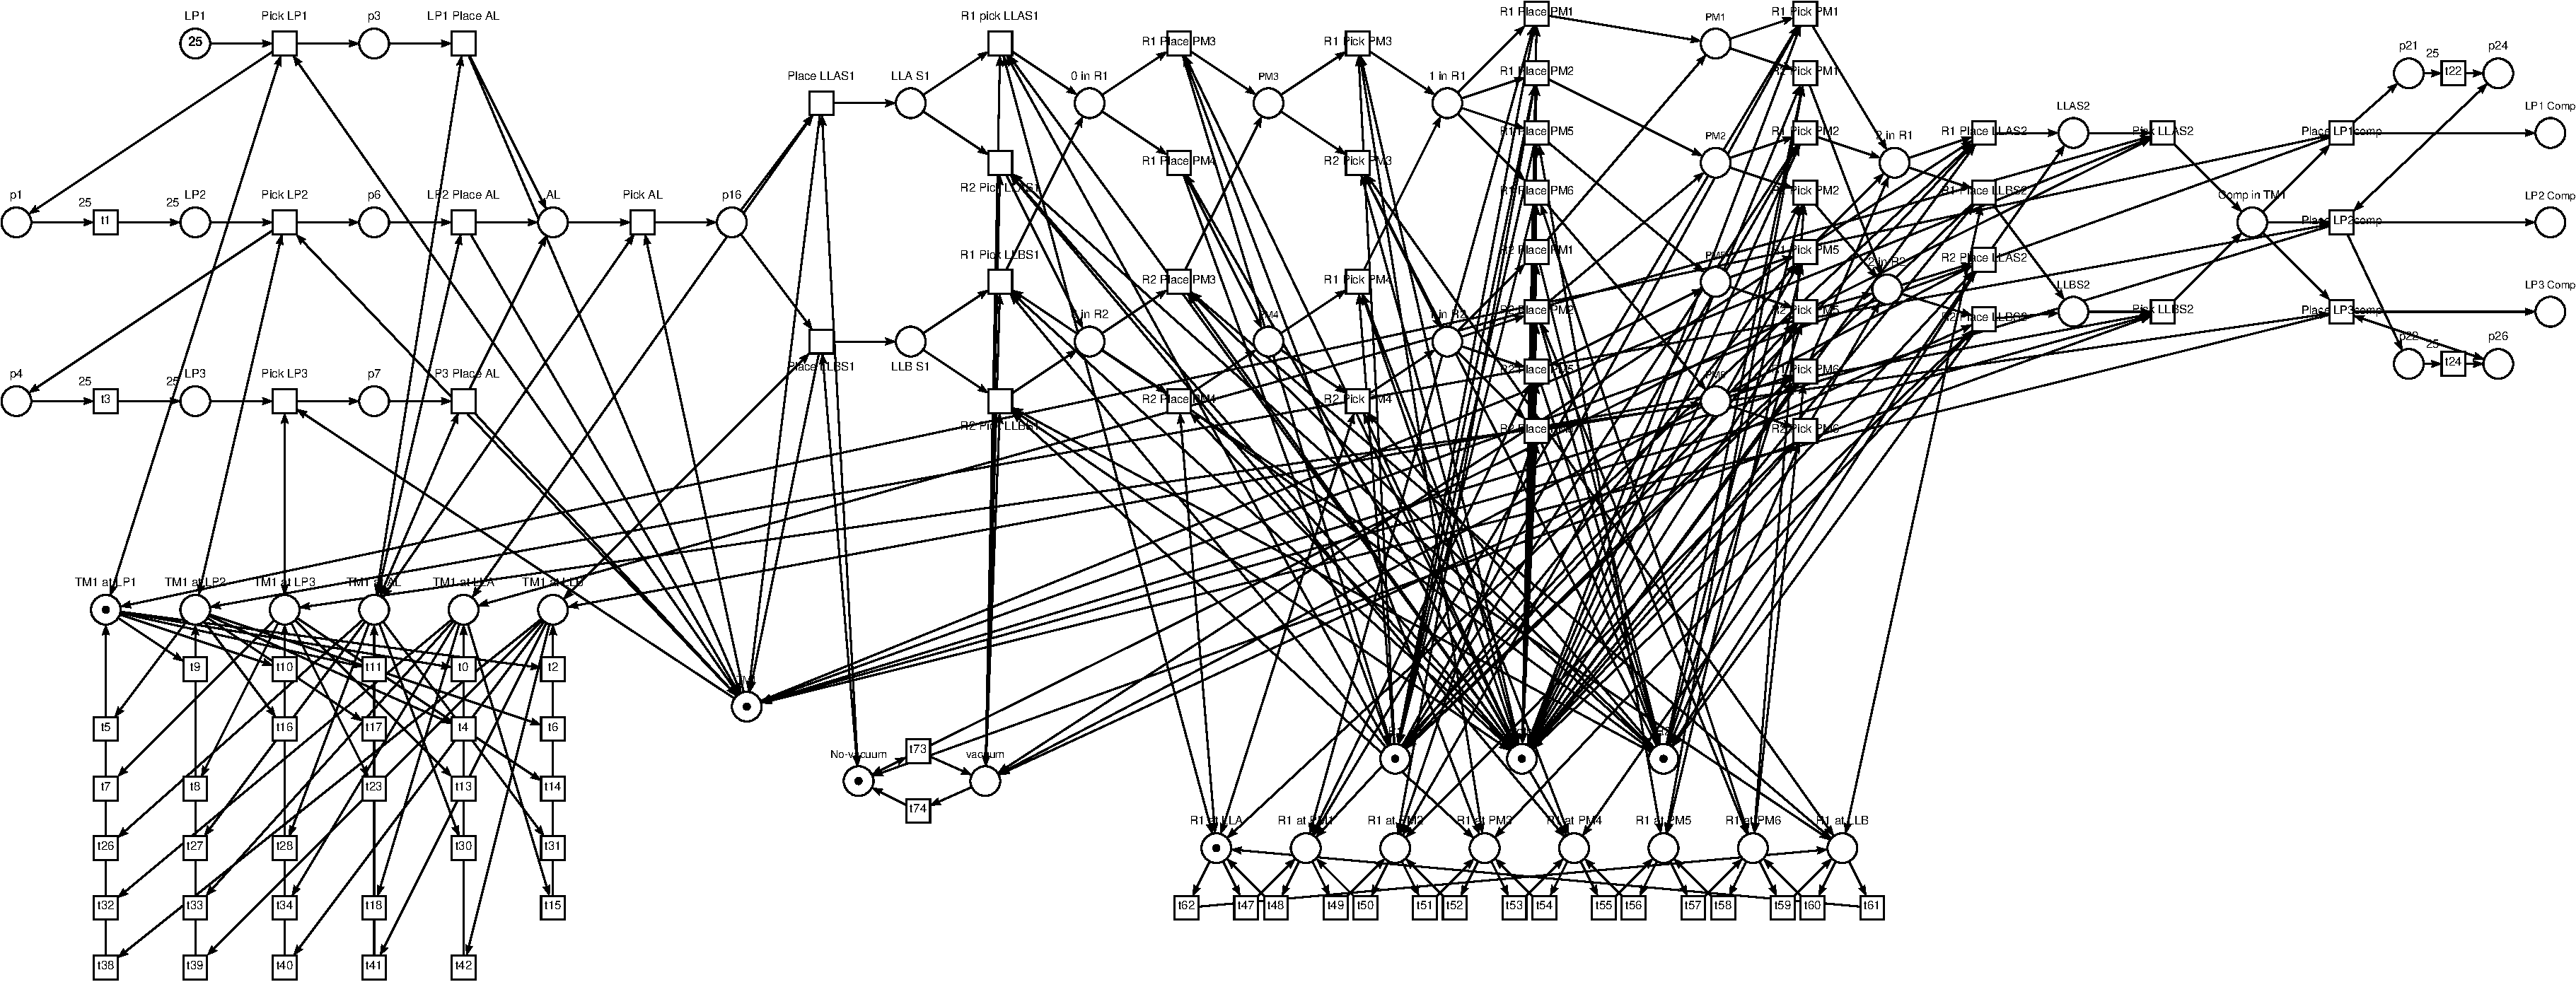
\includegraphics[width=\linewidth]{figures/国赛问题一完全.pdf}\\
	\caption{实际晶圆制造系统}
\end{figure}

本文第四章将使用蚁群算法对此模型进行调度。
\section{本章小结}
本章在上一章的基础上,将库所时间网和变迁时间网结合起来,提出了一种新的时间网子类:库所变迁时间网(TTPPN);
设计了一套TTPPN发射变迁的流程,供下一章的调度算法使用;
设计了一种计算各种Petri网模型的程序架构;
最后使用TTPPN对一个实际的晶圆制造系统进行建模。